\documentclass[11pt]{article}
\usepackage[a4paper,margin=12mm]{geometry}
\usepackage[no-math]{fontspec}
\setmainfont{Latin Modern Roman}
\usepackage{mathtools,amsmath,amssymb,amsfonts,amsthm,xurl}
\usepackage{tikz}
\usetikzlibrary{arrows.meta}
\usepackage[shortlabels]{enumitem}
\usepackage[unicode,hidelinks]{hyperref}
\allowdisplaybreaks
\setlength\emergencystretch{3em}
\newcommand{\ceil}[1]{\left\lceil{#1}\right\rceil}
\newcommand{\abs}[1]{\left\lvert{#1}\right\rvert}
\newcommand{\EE}{\mathbb{E}}
\newcommand{\RR}{\mathbb{R}}
\newcommand{\cC}{\mathcal{C}}
\newcommand{\cS}{\mathcal{S}}
\newcommand{\cT}{\mathcal{T}}
\newcommand{\eps}{\varepsilon}
\newcommand{\ol}[1]{\overline{#1}}
\DeclareMathOperator{\Sol}{Sol}
\definecolor{DarkSlateGray3}{RGB}{121,205,205}
\definecolor{MediumPurple3}{RGB}{137,104,205}
\definecolor{Honeydew3}{RGB}{193,205,193}
\definecolor{Honeydew4}{RGB}{131,139,131}
\newtheorem{theorem}{Theorem}[section]
\newtheorem{lemma}[theorem]{Lemma}
\newtheorem{proposition}[theorem]{Proposition}
\newtheorem{claim}[theorem]{Claim}
\newtheorem{corollary}[theorem]{Corollary}
\newtheorem{definition}[theorem]{Definition}
\newtheorem{example}[theorem]{Example}
\newtheorem{remark}[theorem]{Remark}
\begin{document}\begin{center}\Large Problem2454: Local difference-set upper bounds\end{center}\noindent\textbf{Author:} Sanjana Das\par\noindent\textbf{Work/version:} Bounds for the Local Properties Problem for Difference Sets; Published Discrete Analysis2025:10,45pp.;3September2025; DOI10.19086/da.142094; fresh exact arXiv2310.13999v3 PDF byte-matches saved published original\par\noindent\textbf{Published source/license:} \url{https://arxiv.org/pdf/2310.13999v3}, \url{https://creativecommons.org/licenses/by/3.0/}\par\noindent\textbf{Difficulty:} H2: The proof classifies every local equal-difference configuration by projected solution-space dimensions and removes all heavy configurations from a random subset of a progression-free set. It proves a rank-dependent lower bound for distinct positive differences using a technical certification lemma for linearly independent difference equalities. Minimal linear dependencies are decomposed into overlapping components whose variable counts control every implied repetition, closing the local-property construction.\par\medskip\noindent\textbf{Editorial source boundary:} Theorem1.6 is the sole selected upper-bound family, with its complete positive-absolute-difference convention and every parameter retained. The complete Behrend random alteration, heavy-configuration occurrence count, dimension/repeated-difference bound, minimal-implication variable count, connected-box/blob certification and final closing are included. Proposition1.7 is an unselected statement retained only for literal contextual forward references; neither it nor supporting lemmas/illustrations gets another count. Named Behrend, Chernoff, Markov and elementary linear algebra remain established prerequisites. Printed author text and fully editable Figure2 are checked transcription from the actual CC BY3.0 published version; the matching nonexclusive native archive/classes/private preamble/unprinted comments stay private and unexecuted. Ten finite standard AMS/mathtools names and four independently specified printed colors retain literal author calls and diagram labels. Source Eq10 retains epsilon\_t alongside the complete excluded-tail definition and explicit t-prime equation count; the final blob sum retains p alongside the authored sum through r and each per-box count. These printed discrepancies are disclosed without replacing tokens or supplying a derivation. No mathematical proof, parameter or hypothesis is altered or generated. Root source admission remains required.\par\medskip\hrule\medskip\noindent\textbf{Checked published author text follows.}\par
% Checked published author text; private-aid LF positions133--141
\setcounter{section}{1}\setcounter{subsection}{1}
\subsection{A local properties problem for difference sets}

We study an arithmetic version of such local properties problems, suggested by Zeev Dvir (see \cite{PS19}). We consider sets of real numbers for which every small piece is `arithmetically unstructured,' and we wish to understand how arithmetically unstructured this local property requires the entire set to be. One measure of the extent to which a set is arithmetically structured is the size of its difference set --- roughly, sets with smaller difference set relative to their size possess more arithmetic structure. So we consider sets for which every small subset has a reasonably large difference set, and attempt to understand how large the difference set of the entire set must be. 

We now make this precise. For a set $A \subseteq \RR$, we define the \emph{difference set} of $A$ to be \[A - A = \{\abs{a - b} \mid a, b \in A, \, a \neq b\}.\] Note that we include only positive differences in $A - A$; this definition is somewhat nonstandard but more natural for the problem we study. (When discussing the differences present in a set, we refer only to positive differences, unless otherwise stated.)

For integers $n \geq k \geq 1$ and $\ell \geq 0$, we define $g(n, k, \ell)$ to be the minimum value of $\abs{A - A}$ over all $n$-element sets $A \subseteq \RR$ with the property that every $k$-element subset $A' \subseteq A$ satisfies $\abs{A' - A'} \geq \ell$; we refer to this property as the \emph{$(k, \ell)$-local property}. (Note that the same definition can be used to define $g(n, k, \ell)$ even when $\ell$ is not a nonnegative integer; then $g(n, k, \ell) = g(n, k, \ceil{\ell})$. This makes certain results slightly more convenient to state.) We think of $k$ and $\ell$ as fixed and $n$ as large, and we study the asymptotic behavior of $g(n, k, \ell)$ as $n$ tends to infinity. (In particular, in all asymptotic notation in this paper, $n$ tends to infinity while all other quantities are fixed; the implied constants may depend on $k$, $\ell$, and any other stated parameters.)

As with the local properties problem for graph colorings, we can attempt to understand $g(n, k, \ell)$ either by fixing $\ell$, or by considering various thresholds. Note that for all $n$-element sets $A \subseteq \RR$ we have $n - 1 \leq \abs{A - A} \leq \binom{n}{2}$ (and $\abs{A - A} = n - 1$ if and only if $A$ is an arithmetic progression), so for all $\ell \leq \binom{k}{2}$ we have \[n - 1 \leq g(n, k, \ell) \leq \binom{n}{2}.\] (If $\ell > \binom{k}{2}$, then no set $A$ can satisfy the $(k, \ell)$-local property, so we say that $g(n, k, \ell) = +\infty$.) Also note that $g(n, k, \ell)$ is weakly increasing in $\ell$, as increasing $\ell$ only makes the $(k, \ell)$-local property stronger. So it is natural to consider, for fixed $k$, how long $g(n, k, \ell)$ stays linear and when it becomes quadratic as we increase $\ell$. To formalize this, as defined in \cite{Li22}, the \emph{superlinear threshold} is defined to be the largest integer $\ell$ (as a function of $k$) such that $g(n, k, \ell) = O(n)$, and the \emph{quadratic threshold} is defined to be the smallest integer $\ell$ (as a function of $k$) such that $g(n, k, \ell) = \Omega(n^2)$. (Note that $g(n, k, k - 1) = n - 1$, so at the superlinear threshold we actually have $g(n, k, \ell) = \Theta(n)$; similarly, if $k \geq 4$ then $g(n, k, \binom{k}{2}) = \binom{n}{2}$, so at the quadratic threshold we actually have $g(n, k, \ell) = \Theta(n^2)$.)  
% Checked published author text; private-aid LF positions196--200
\setcounter{theorem}{5}
We now state our more general theorems from which we deduce these statements. First, we prove the following family of upper bounds for $g(n, k, \ell)$. 

\begin{theorem}\label{thm:upper-bound}
    For all positive integers $k$ and all $1 < c \leq 2$, we have \[g\left(n, k, \ceil{\frac{(c - 1)(k - 1)}{c}}^2\right) = o(n^c).\] 
\end{theorem}
% Checked published author text; private-aid LF positions204--208

\begin{proposition}\label{prop:odd-upper-bound}
    For all odd positive integers $k$, we have \[g\left(n, k, \frac{(k + 1)^2}{4} - 4\right) = o(n^2).\] 
\end{proposition}

We obtain Theorem \ref{thm:upper-bound} and Proposition \ref{prop:odd-upper-bound} by using a random construction. To ensure that the constructed set satisfies the $(k, \ell)$-local property for the stated values of $\ell$, we consider all possible `configurations' of equal differences that can be formed by a $k$-element subset. We first show, very roughly, that certain `bad' configurations are expected to occur very few times in the random construction, so using the alteration method, we can ensure that our set only contains `good' configurations. We then show that any $k$-element subset forming a good configuration must contain at least $\ell$ distinct differences. The technical steps of our proof rely on considering the systems of equations associated with such configurations and analyzing their linear algebraic properties. 
% Checked published author text; private-aid LF positions269--547
\setcounter{section}{1}\setcounter{equation}{4}\setcounter{figure}{1}
\section{Proof of Theorem \ref{thm:upper-bound}: A family of upper bounds on \texorpdfstring{$g(n, k, \ell)$}{g(n, k, l)}} \label{sec:upper-bound}

In this section, we prove Theorem \ref{thm:upper-bound} (our family of upper bounds). The structure of the proof is as follows: let $\ell$ be as in Theorem \ref{thm:upper-bound}. In order to show that $g(n, k, \ell) = o(n^c)$, we need to show that for all $a > 0$, for all sufficiently large $n$ we have $g(n, k, \ell) \leq an^c$ --- i.e., there exists an $n$-element set $A \subseteq \RR$ with $\abs{A - A} \leq an^c$ satisfying the $(k, \ell)$-local property. We will obtain such a set $A$ using a random construction. In order to ensure that our set $A$ satisfies the $(k, \ell)$-local property, for every $k$-element subset $A' \subseteq A$, we consider the `configuration' of equal differences formed by its elements. Our argument will then consist of two steps: first, we show that using a random construction, we can obtain an $n$-element set $A$ with $\abs{A - A} \leq an^c$ that avoids all `bad' configurations (where we classify configurations as good or bad based on certain properties). We then show that any $k$-element subset forming a `good' configuration necessarily contains at least $\ell$ distinct differences. It then follows that the set $A$ we constructed must satisfy the $(k, \ell)$-local property, providing the desired upper bound. 

In Subsection \ref{subsec:setup}, we set up a few useful definitions (in particular, we formalize the notion of a configuration of equal differences) and state these two steps more precisely (with definitions of which configurations we consider good and bad). In Subsection \ref{subsec:random-construct}, we describe our random construction and prove that it avoids all bad configurations. In Subsection \ref{subsec:bounding-diffs}, we prove that any subset forming a good configuration contains at least $\ell$ distinct differences, modulo a certain technical lemma; in Subsection \ref{subsec:2s-certify}, we prove this lemma. 

\subsection{Setup} \label{subsec:setup} 

We formalize the notion of a configuration of equal differences in the following way: we define a \emph{$k$-configuration} to be a collection of linear equations over $\RR$ in the $k$ variables $x_1$, \ldots, $x_k$, in which each equation is of the form \begin{align}
    x_{i_1} - x_{i_2} - x_{i_3} + x_{i_4} = 0 \label{eqn:generic-diffeq}
\end{align} 
for some (not necessarily distinct) indices $i_1, i_2, i_3, i_4 \in \{1, \ldots, k\}$ such that $\{i_1, i_4\} \neq \{i_2, i_3\}$. We refer to such an equation as a \emph{difference equality}. (The name, as well as the reason we care about such equations, comes from the fact that \eqref{eqn:generic-diffeq} is a rearrangement of $x_{i_1} - x_{i_2} = x_{i_3} - x_{i_4}$. The condition $\{i_1, i_4\} \neq \{i_2, i_3\}$ means that we only consider equations that are not identically satisfied.) 

In the remainder of this subsection, we establish some useful definitions regarding $k$-configurations; using these definitions, we then state our two main steps more precisely, as Lemmas \ref{lem:random-construct} and \ref{lem:bounding-diffs}. 

\subsubsection{Conventions} 

We first fix a few conventions regarding linear equations (working over the field $\RR$). 

We consider equations to be unique only up to rearrangement; for example, we consider \eqref{eqn:generic-diffeq} to be the same equation as $-x_{i_1} + x_{i_2} + x_{i_3} - x_{i_4} = 0$, $x_{i_1} - x_{i_2} = x_{i_3} - x_{i_4}$, and $x_{i_1} + x_{i_4} = x_{i_2} + x_{i_3}$. 

Given a linear equation $(*)$ in $x_1$, \ldots, $x_k$, we define its \emph{content} to be an expression $*$ (which is a linear combination of $x_1$, \ldots, $x_k$) such that $(*)$ is the equation ${*} = 0$. (For any nontrivial equation $(*)$, there are two ways to define the content of $(*)$, where each is the negative of the other; we choose one arbitrarily.) For example, the content of the difference equality \eqref{eqn:generic-diffeq} is either $x_{i_1} - x_{i_2} - x_{i_3} + x_{i_4}$ or its negative.

We say that a variable $x_i$ \emph{appears} in a linear equation $(*)$, or that $(*)$ \emph{involves} $x_i$, if the coefficient of $x_i$ in $(*)$ is nonzero. (For example, the equation $x_1 - x_2 = 0$ involves $x_1$ and $x_2$, but does not involve $x_3$; this remains the case even if we write it as $x_1 - x_2 - x_3 + x_3 = 0$.)  We also use the same terminology for linear expressions $*$ in place of linear equations $(*)$. Given a set $I \subseteq \{1, \ldots, k\}$, we say $(*)$ is an \emph{equation on $I$} if all variables $x_i$ appearing in $(*)$ satisfy $i \in I$. 

We say linear equations $(*_1)$, \ldots, $(*_t)$ are \emph{linearly independent} if their contents $*_1$, \ldots, $*_t$ are linearly independent (viewed as elements of the $k$-dimensional $\RR$-vector space with basis vectors $x_1$, \ldots, $x_k$). 

Given linear equations $(*_1)$, \ldots, $(*_t)$, $(*)$ with contents $*_1$, \ldots, $*_t$, $*$, we say that the collection $\cT = \{(*_1), \ldots, (*_t)\}$ \emph{implies} $(*)$ if $*$ can be written as a linear combination of $*_1$, \ldots, $*_t$, i.e., \[{*} = \eps_1{*_1} + \cdots + \eps_t{*_t}\] for some $\eps_1, \ldots, \eps_t \in \RR$. (The reason for this terminology is that this is equivalent to the condition that every solution to $\cT$ (viewed as a system of equations) is also a solution to $(*)$; however, we will not need this fact.) We say $\cT$ \emph{minimally implies} $(*)$ if $\cT$ implies $(*)$, but no proper subset $\cT' \subset \cT$ does. (Equivalently, $\cT$ minimally implies $(*)$ if and only if $(*_1)$, \ldots, $(*_t)$ are linearly independent and the coefficients $\eps_1$, \ldots, $\eps_t$ above are all nonzero.) 

We say two collections of linear equations $\cC_1$ and $\cC_2$ are \emph{equivalent} if $\cC_1$ implies every equation in $\cC_2$, and $\cC_2$ implies every equation in $\cC_1$. 

\subsubsection{Definitions for \texorpdfstring{$k$}{k}-configurations}

For a $k$-configuration $\cC$, we let $\Sol(\cC) \subseteq \RR^k$ denote the set of solutions to $\cC$ (where we view $\cC$ as a system of linear equations over $\RR$). For each $I \subseteq \{1, \ldots, k\}$, we let $\Sol_I(\cC)$ denote the projection of $\Sol(\cC)$ onto the coordinates in $I$ --- in other words, we define \[\Sol_I(\cC) = \{(x_i)_{i \in I} \mid (x_1, \ldots, x_k) \in \Sol(\cC)\}.\] We refer to the elements of $\Sol_I(\cC)$ as \emph{$I$-solutions to $\cC$}. 

We define the \emph{dimension} of $\cC$, denoted $\dim(\cC)$, to be the dimension of $\Sol(\cC)$ as a $\RR$-vector space; similarly, for each $I \subseteq \{1, \ldots, k\}$, we define $\dim_I(\cC)$ to be the dimension of $\Sol_I(\cC)$. 

We say a solution to $\cC$ is \emph{generic} if it does not satisfy any difference equalities other than the ones implied by $\cC$. Of course, any solution to $\cC$ must satisfy all equations implied by $\cC$, so a generic solution to $\cC$ satisfies all the difference equalities implied by $\cC$ and no others. (This definition will be used to encapsulate what we mean by a $k$-element set `forming' a configuration of equal differences, as stated in the outline in the beginning of Section \ref{sec:upper-bound}.)

We define an \emph{occurrence} of a $k$-configuration $\cC$ in a set $A \subseteq \RR$ to be a solution to $\cC$ consisting of \emph{distinct} elements of $A$; if there is an occurrence of $\cC$ in $A$, we say $\cC$ \emph{occurs} in $A$. For $I \subseteq \{1, \ldots, k\}$, we define an \emph{$I$-occurrence} of $\cC$ to be an $I$-solution to $\cC$ consisting of distinct elements of $A$. 

\begin{example}
    We illustrate these definitions for the $6$-configuration \[\cC = \{x_1 - x_2 - x_3 + x_4 = 0, \, x_1 - x_2 - x_5 + x_6 = 0\}.\]
    \begin{itemize}
        \item We have $\dim(\cC) = 4$ --- to obtain a solution to $\cC$, we can choose $x_1$, $x_2$, $x_3$, and $x_5$ arbitrarily, and then $x_4$ and $x_6$ are uniquely determined. For the same reason, we have $\dim_{\{1, 2, 3, 5\}}(\cC) = 4$ and $\dim_{\{1, 2, 3, 4\}}(\cC) = 3$ (as $x_4$ is uniquely determined by $x_1$, $x_2$, and $x_3$). Similarly, we have $\dim_{\{3, 4, 5, 6\}}(\cC) = 3$ --- this is because $\cC$ implies $x_3 - x_4 - x_5 + x_6 = 0$, so we can choose $x_3$, $x_4$, and $x_5$ arbitrarily, and then $x_6$ is uniquely determined. 
        \item The $6$-tuple $(1, 2, 4, 5, 9, 10)$ is a solution to $\cC$, but it is not generic, as it satisfies the additional difference equality $x_1 - x_4 = x_4 - x_5$. By contrast, $(1, 2, 4, 5, 10, 11)$ is a generic solution to $\cC$.  
        \item Consider the set $A = \{1, 2, 4, 5, 9, 10, 11\}$. Then $(1, 2, 4, 5, 9, 10)$ and $(1, 2, 4, 5, 10, 11)$ are both occurrences of $\cC$ in $A$. Any $4$-tuple of distinct elements of $A$ is a $\{1, 2, 3, 5\}$-occurrence of $\cC$ in $A$, and $(1, 10, 2, 11)$ is a $\{1, 2, 3, 4\}$-occurrence and a $\{3, 4, 5, 6\}$-occurrence of $\cC$ in $A$. 
    \end{itemize}
\end{example}

We are now ready to define the properties of a $k$-configuration that determine whether we consider them `good' or `bad' (as in the outline of our argument given at the beginning of Section \ref{sec:upper-bound}). 

First, we say that a $k$-configuration is \emph{invalid} if it implies $x_{i_1} - x_{i_2} = 0$ for some $i_1 \neq i_2$ (i.e., it implies two variables are equal), and \emph{valid} otherwise. Note that an invalid $k$-configuration can never occur in a set $A$ (because of the distinctness condition in the definition of an occurrence). Also note that in a generic solution to a valid $k$-configuration, all $k$ entries must be distinct. 

We say a $k$-configuration is \emph{AP-containing} if it implies $x_{i_1} - 2x_{i_2} + x_{i_3} = 0$ for some distinct $i_1$, $i_2$, $i_3$ (i.e., it implies three variables form an arithmetic progression), and \emph{AP-free} otherwise. 

Most importantly, given any $1 < c \leq 2$, we say a $k$-configuration $\cC$ is \emph{$c$-heavy} if there exists some $1 \leq m \leq k$ and some $m$-element subset $I \subseteq \{1, \ldots, k\}$ such that \[\dim_I(\cC) < \frac{(c - 1)m + 1}{c},\] and we call such a subset $I$ a \emph{$c$-heavy part} of $\cC$; we say $\cC$ is \emph{$c$-light} if it is not $c$-heavy. (This definition was chosen in order to make the expected value calculation in the proof of Claim \ref{claim:heavy-occs} work out.)

\begin{remark}\label{rmk:c-light-alt}
    Note that if $\cC$ is $c$-light, then for any $I \subseteq \{1, \ldots, k\}$ of size $\abs{I} = m$, any collection of linearly independent equations on $I$ implied by $\cC$ has size at most \[m - \dim_I(\cC) \leq m - \frac{(c - 1)m + 1}{c} = \frac{m - 1}{c}.\] Equivalently, any collection of $t$ linearly independent equations implied by $\cC$ must involve at least $ct + 1$ variables. We will use this observation frequently in our proof of Proposition \ref{prop:odd-upper-bound} (with $c = 2$). 
\end{remark}

Finally, we say a $k$-configuration $\cC$ is \emph{$c$-good} if it is valid, AP-free, and $c$-light; we say it is \emph{$c$-bad} otherwise. Note that if a $k$-configuration $\cC$ has any of these three properties (i.e., is valid, AP-free, or $c$-light), then any collection of difference equalities implied by $\cC$ has the same property. 

\begin{example}\label{ex:2-good-illustrate}
    To illustrate these definitions, we consider a few examples with $c = 2$. 
    \begin{enumerate}[(a)]
        \item The $4$-configuration $\{x_1 - x_2 - x_3 + x_4 = 0, \, x_1 - x_2 + x_3 - x_4 = 0\}$ is invalid, because it implies $x_3 = x_4$. (It is also $2$-heavy, with both $\{3, 4\}$ and $\{1, 2, 3, 4\}$ as $2$-heavy parts.) 
        \item The $5$-configuration $\{x_1 - x_2 - x_3 + x_4 = 0, \, x_1 + x_2 - x_3 - x_5 = 0\}$ is valid and $2$-light, but it is AP-containing (as it implies $x_5 - 2x_2 + x_4 = 0$) and therefore $2$-bad. 
        \item The $12$-configuration $\{x_1 - x_2 - x_3 + x_4 = 0, \, x_1 - x_2 - x_5 + x_6 = 0, \, x_1 - x_2 - x_7 + x_8 = 0, \, x_1 - x_3 - x_5 + x_7 = 0, \, x_9 - x_{10} - x_{11} + x_{12} = 0\}$ is valid and AP-free, but it is $2$-heavy with $2$-heavy part $\{1, \ldots, 8\}$ (as it contains $4$ linearly independent equations on $\{1, \ldots, 8\}$), and therefore $2$-bad. 
        \item \label{item:ex-2-good} The $6$-configuration $\cC = \{x_1 - x_2 - x_5 + x_4 = 0, \, x_1 - x_3 - x_6 + x_4 = 0\}$ --- equivalently, $\{x_1 + x_4 = x_2 + x_5 = x_3 + x_6\}$ --- is $2$-good, as it is valid, AP-free, and $2$-light. The fact that it is $2$-light can be seen by pairing $x_1$ and $x_4$, $x_2$ and $x_5$, and $x_3$ and $x_6$ --- we can obtain the solutions to $\cC$ by freely choosing the values of both variables in one pair and one variable in each of the other pairs (then the values of the remaining two variables are uniquely determined), and for any $I \subseteq \{1, \ldots, 6\}$ of size $m \geq 1$, this gives a way of freely choosing the values of more than half of the variables $x_i$ with indices $i \in I$, thus showing that $\dim_I(\cC) \geq \frac{m + 1}{2}$. 
    \end{enumerate}
\end{example}

\subsubsection{Our main steps}

Finally, we state the results of the two main steps of our argument as lemmas and explain why they imply Theorem \ref{thm:upper-bound}. 

The following lemma will be the result of the first step of our argument, where we use a random construction to obtain a set $A$ with few distinct differences that `avoids' all $c$-bad $k$-configurations.

\begin{lemma} \label{lem:random-construct}
    Fix a positive integer $k$ and real numbers $1 < c \leq 2$ and $a > 0$. Then for all sufficiently large $n$ (with respect to $k$, $c$, and $a$), there exists an $n$-element set $A \subseteq \RR$ with $\abs{A - A} \leq an^c$ such that every $k$-configuration that occurs in $A$ is $c$-good. 
\end{lemma}

The following lemma will be the result of the second step of our argument, in which we show that a generic solution to a $c$-good $k$-configuration contains many distinct differences. In fact, we show more generally that a generic solution to any valid $k$-configuration with high dimension contains many distinct differences. 

\begin{lemma} \label{lem:bounding-diffs}
    Fix a positive integer $k$, let $\cC$ be a valid $k$-configuration, and let $\dim(\cC) = d$. Let $(a_1, \ldots, a_k)$ be a generic solution to $\cC$, and let $A' = \{a_1, \ldots, a_k\}$. Then 
    \begin{align} 
        \abs{A' - A'} \geq \begin{cases} (d - 1)^2 & \text{if $d \leq \frac{k}{2} + 1$} \\ \binom{k}{2} - (k - d)(k - d + 1) & \text{if $d \geq \frac{k}{2} + 1$}.\end{cases} \label{eqn:bounding-diffs-bound}
    \end{align}
\end{lemma}

Note that the two expressions in \eqref{eqn:bounding-diffs-bound} are equal at $d = \frac{k}{2} + 1$, and both are (weakly) increasing in $d$; this means that the entire right-hand side of \eqref{eqn:bounding-diffs-bound} is increasing in $d$. 

We will prove these two lemmas in Subsections \ref{subsec:random-construct} and \ref{subsec:bounding-diffs}, respectively. For now, we explain why they together imply Theorem \ref{thm:upper-bound}. 

\begin{proof}[Proof of Theorem \ref{thm:upper-bound}]
    By the comments at the beginning of Section \ref{sec:upper-bound}, it suffices to show that the sets $A$ given by Lemma \ref{lem:random-construct} satisfy the $(k, \ell)$-local property for the value of $\ell$ in Theorem \ref{thm:upper-bound}. To see this, suppose that a set $A$ has the property that every $k$-configuration occurring in $A$ is $c$-good. Then for any $k$-element subset $A' = \{a_1, \ldots, a_k\} \subseteq A$, we can write down the $k$-configuration $\cC$ consisting of \emph{all} the difference equalities satisfied by $(a_1, \ldots, a_k)$. Then $\cC$ occurs in $A$, so it must be $c$-good; in particular, $\cC$ is valid and \[\dim(\cC) \geq \ceil{\frac{(c - 1)k + 1}{c}}\] (by the $c$-light condition applied to the entire set $\{1, \ldots, k\}$, and the fact that $\dim(\cC)$ is an integer). Meanwhile $(a_1, \ldots, a_k)$ is a generic solution to $\cC$ (as every difference equality it satisfies is in fact \emph{contained} in $\cC$), so we can bound $\abs{A' - A'}$ using Lemma \ref{lem:bounding-diffs}. The bound given by \eqref{eqn:bounding-diffs-bound} is increasing in $d$ and we have \[\ceil{\frac{(c - 1)k + 1}{c}} \leq \ceil{\frac{k + 1}{2}} \leq \frac{k}{2} + 1,\] so Lemma \ref{lem:bounding-diffs} gives that \[\abs{A' - A'} \geq \left(\ceil{\frac{(c - 1)k + 1}{c}} - 1\right)^2 = \ceil{\frac{(c - 1)(k - 1)}{c}}^2 = \ell.\] This means $A$ indeed satisfies the $(k, \ell)$-local property, as desired. 
\end{proof}

\begin{remark}
    For this argument, we do not need the full strength of Lemma \ref{lem:random-construct} --- the only parts of the $c$-good condition that we need are that a $c$-good configuration $\cC$ is valid and satisfies $\dim(\cC) \geq \frac{(c - 1)k + 1}{c}$. However, we will need the remaining parts of the $c$-good condition in our proof of Proposition \ref{prop:odd-upper-bound} (and we state Lemma \ref{lem:random-construct} in this way so that we can use it for that proof as well).
\end{remark}

\subsection{Proof of Lemma \ref{lem:random-construct}} \label{subsec:random-construct}

In this subsection, we prove Lemma \ref{lem:random-construct} using a random construction (with the alteration method). Our construction will make use of the following theorem of Behrend. 

\begin{theorem}[Behrend \cite{Beh46}]\label{thm:behrend}
    For every positive integer $n$, there exists a set $S \subseteq \{1, \ldots, n\}$ of size $\abs{S} = n^{1 - o(1)}$ containing no $3$-term arithmetic progression. 
\end{theorem}

\begin{proof}[Proof of Lemma \ref{lem:random-construct}]
    Assume that $n$ is sufficiently large with respect to $k$, $c$, and $a$ (all our asymptotic notation treats $k$, $c$, and $a$ as fixed, and the implied constants will depend on them). First, by Theorem \ref{thm:behrend}, there exists a set $S \subseteq \{1, \ldots, \ceil{an^c}\}$ of size $s = n^{c - o(1)}$ with no $3$-term arithmetic progression. We will ultimately take $A$ to be an $n$-element subset of $S$, which will automatically imply that $\abs{A - A} \leq an^c$ (as we have $A - A \subseteq S - S \subseteq \{1, \ldots, \ceil{an^c} - 1\}$) and that every $k$-configuration that occurs in $A$ is AP-free. So in order to prove Lemma \ref{lem:random-construct}, it will suffice to ensure that every $k$-configuration that occurs in $A$ is $c$-light. (We automatically have that every $k$-configuration that occurs in $A$ is valid, as this is true for \emph{any} set.)

    Let $p = \frac{3n}{s}$. Note that $p = n^{1 - c + o(1)}$, so $p \in (0, 1)$ for all sufficiently large $n$. Let $T$ be a randomly chosen subset of $S$ where each element is included independently with probability $p$. Then $\EE[\abs{T}] = 3n$, and since $\abs{T}$ is a sum of $s$ independent Bernoulli random variables, by the Chernoff bounds we have $\abs{T} \geq 2n$ with probability $1 - o(1)$. 

    We will show that with probability $1 - o(1)$, it is possible to destroy all occurrences of $c$-heavy $k$-configurations in $T$ by deleting at most $n$ of its elements (which we will then do to obtain our set $A$). The following claim allows us to do so. 

    \begin{claim}\label{claim:heavy-occs}
        Let $\cC$ be a $c$-heavy $k$-configuration, and let $I$ be a $c$-heavy part of $\cC$. Then the expected number of $I$-occurrences of $\cC$ in $T$ is $o(n)$. 
    \end{claim}

    \begin{proof}
        Let $d = \dim_I(\cC)$. First, we claim that there are at most $s^d$ $I$-occurrences of $\cC$ in $S$. To see this, without loss of generality assume $I = \{1, \ldots, m\}$ for some $m$. By solving $\cC$ using reduced row echelon form, we can find a list of indices $i_1 < \cdots < i_{d'}$, where $d' = \dim(\cC)$, such that every choice of values for $x_{i_1}$, \ldots, $x_{i_{d'}}$ in $\RR$ corresponds to a unique solution $(x_1, \ldots, x_k)$ to $\cC$, and for each $i \in \{1, \ldots, k\}$, the value of $x_i$ in this solution depends on only the chosen values of $x_{i_j}$ for the indices $i_j < i$. Then each choice of values for $x_{i_j}$ over all indices $i_j \leq m$ corresponds to a unique $I$-solution to $\cC$, so there must be exactly $\dim_I(\cC) = d$ such indices. Finally, each choice of values for these $d$ variables $x_{i_j}$ in $S$ provides at most one $I$-solution to $\cC$ whose elements are in $S$, and therefore at most one $I$-occurrence of $\cC$ in $S$. There are $s^d$ such choices, so there are at most $s^d$ $I$-occurrences of $\cC$ in $S$. 

        Now for each $I$-occurrence of $\cC$ in $S$, the probability that all its elements are included in $T$ is $p^m$ (as it has $m$ distinct elements, each of which is included in $T$ independently with probability $p$). So by the linearity of expectation, the expected number of $I$-occurrences of $\cC$ in $T$ is at most $s^d \cdot p^m$. Since $s = n^{c - o(1)}$ and $p = n^{1 - c + o(1)}$, we have \[s^d \cdot p^m = n^{cd + m(1 - c) + o(1)}.\] Since $cd + m(1 - c) < 1$ by the definition of a $c$-heavy part (and this quantity is a constant not depending on $n$), we have $s^d \cdot p^m = o(n)$, as desired. 
    \end{proof}

    Now for each $c$-heavy $k$-configuration $\cC$, fix some $c$-heavy part of $\cC$, which we denote by $h(\cC)$. Then Claim \ref{claim:heavy-occs} implies that for each \emph{fixed} $c$-heavy $\cC$, the number of $h(\cC)$-occurrences of $\cC$ in $T$ has expected value $o(n)$. But the total number of $k$-configurations is a constant (depending on $k$ but not $n$), since for any given $k$, there are only finitely many difference equalities. So the \emph{total} number of $h(\cC)$-occurrences of $\cC$ over all $c$-heavy $\cC$ has expected value $o(n)$ as well. Then by Markov's inequality, this number is at most $n$ with probability $1 - o(1)$. 

    So with probability $1 - o(1)$, we have $\abs{T} \geq 2n$ and there are at most $n$ total $h(\cC)$-occurrences of $\cC$ in $T$ over all $c$-heavy $k$-configurations $\cC$; this means that for sufficiently large $n$, there must exist a set $T \subseteq S$ with both properties. Fix such a set $T$, and let $A$ be an $n$-element subset of $T$ obtained by first deleting some element from each $h(\cC)$-occurrences of each $c$-heavy $\cC$ (which requires us to delete at most $n$ elements), and then deleting additional elements arbitrarily until we are left with exactly $n$ elements. 

    We have already shown that $\abs{A - A} \leq an^c$ and that no invalid or AP-containing $k$-configuration can occur in $A$; this construction guarantees that no $c$-heavy $k$-configuration can occur in $A$ (as any occurrence of a $c$-heavy $k$-configuration $\cC$ would contain a $h(\cC)$-occurrence of $\cC$). So $A$ has all the claimed properties. 
\end{proof}

\subsection{Proof of Lemma \ref{lem:bounding-diffs}} \label{subsec:bounding-diffs}

In this subsection, we prove Lemma \ref{lem:bounding-diffs} (our lower bound on the number of distinct differences in a generic solution to a valid $k$-configuration, in terms of the dimension of the $k$-configuration). We first establish a few definitions that will be useful in this proof. 

Note that equations of the form $x_{i_1} - x_{i_2} = 0$, $2x_{i_1} - 2x_{i_2} = 0$, and $x_{i_1} - 2x_{i_2} + x_{i_3} = 0$ are all considered to be difference equalities, since we do not require the indices in \eqref{eqn:generic-diffeq} to be distinct. We say a difference equality is \emph{degenerate} if it is of the form $x_{i_1} - x_{i_2} = 0$ for distinct indices $i_1$ and $i_2$ (equivalently, in \eqref{eqn:generic-diffeq} the sets $\{i_1, i_4\}$ and $\{i_2, i_3\}$ are different but not disjoint), and \emph{nondegenerate} otherwise. (Since we assume the $k$-configuration $\cC$ we work with is valid, all difference equalities it implies will be nondegenerate.)

Given a nondegenerate difference equality $(*)$, we say that two variables $x_i$ and $x_j$ appear in $(*)$ \emph{with opposite sign} if $(*)$ can be written as $x_i - x_j = x_{i'} - x_{j'}$ for some $i', j' \in \{1, \ldots, k\}$, and \emph{with the same sign} if $(*)$ can be written as $x_i + x_j = x_{i'} + x_{j'}$ for some $i', j' \in \{1, \ldots, k\}$. This definition matches the intuitive meaning of these terms; in the difference equality \eqref{eqn:generic-diffeq}, $x_{i_1}$ appears with opposite sign as both $x_{i_2}$ and $x_{i_3}$, and with the same sign as $x_{i_4}$. 

Given distinct indices $i, j \in \{1, \ldots, k\}$, we say that a collection of linear equations \emph{$i$-certifies $j$} if it implies some nondegenerate difference equality in which $x_i$ and $x_j$ appear with opposite sign. (In particular, we say a single difference equality $i$-certifies $j$ if $x_i$ and $x_j$ appear in it with opposite sign.) 

Our proof of Lemma \ref{lem:bounding-diffs} will require the following lemma. The proof of this lemma is somewhat technical, so we defer it to Subsection \ref{subsec:2s-certify} (and first prove Lemma \ref{lem:bounding-diffs} assuming this lemma). 

\begin{lemma}\label{lem:2s-certify}
    Fix $i \in \{1, \ldots, k\}$, and let $\cS$ be a valid collection of linearly independent difference equalities that all involve $x_i$. Then $\cS$ $i$-certifies at most $2\abs{\cS}$ indices. 
\end{lemma}

\begin{proof}[Proof of Lemma \ref{lem:bounding-diffs}]
    We first make a convenient assumption on the ordering of the indices of $x_1$, \ldots, $x_k$: by using reduced row echelon form to solve $\cC$ (as a system of equations), we can find $d$ distinct indices $i_1$, \ldots, $i_d$ such that every choice of values for $x_{i_1}$, \ldots, $x_{i_d}$ gives a unique solution $(x_1, \ldots, x_k)$ to $\cC$. We assume without loss of generality that these indices are $1$, \ldots, $d$. 

    We can calculate $\abs{A' - A'}$ in the following way: for each pair of indices $(i, j)$ with $1 \leq j < i \leq k$, we say $(i, j)$ corresponds to a \emph{repeated difference} if $\abs{a_i - a_j} = \abs{a_{i'} - a_{j'}}$ for some $(i', j')$ with $1 \leq j' < i' \leq k$ that is lexicographically smaller than $(i, j)$ (i.e., either $i' < i$, or $i' = i$ and $j' < j$), and a \emph{new difference} otherwise. Note that if a pair $(i, j)$ corresponds to a repeated difference, then $(a_1, \ldots, a_k)$ satisfies a nondegenerate difference equality of the form 
    \begin{align}
        x_i - x_j - x_{i'} + x_{j'} = 0\label{eqn:rep-diff}
    \end{align} 
    for some $i', j' \leq i$ (here we do not necessarily have $j' < i'$) --- i.e., a difference equality on $\{1, \ldots, i\}$ in which $x_i$ and $x_j$ occur with opposite sign. Since $(a_1, \ldots, a_k)$ is a generic solution to $\cC$, this difference equality \eqref{eqn:rep-diff} must be implied by $\cC$.
    
    Then $\abs{A' - A'}$ is precisely the number of pairs $(i, j)$ corresponding to new differences. For each index $i$, we will upper-bound the number of repeated differences contributed by $i$ (i.e., the number of indices $j < i$ for which $(i, j)$ corresponds to a repeated difference) by bounding the number of indices $j < i$ for which $\cC$ can imply a difference equality of the form \eqref{eqn:rep-diff}. Combining these bounds over all $i$ will then give the desired lower bound on $\abs{A' - A'}$. 
    
    We first consider the indices $i \leq d$. Our assumption that every choice of $x_1$, \ldots, $x_d$ corresponds to a solution to $\cC$ means that $\cC$ cannot imply any equation on $\{1, \ldots, d\}$, and therefore cannot imply a difference equality of the form \eqref{eqn:rep-diff} for any $j < i \leq d$. So each index $i \leq d$ contributes no repeated differences.

    We now consider the indices $i > d$. Fix some index $i > d$, let $\ol{\cS_i}$ be the set of all difference equalities on $\{1, \ldots, i\}$ involving $x_i$ that are implied by $\cC$, and let $\cS_i$ be a maximal linearly independent subset of $\ol{\cS_i}$. Then $\cS_i$ implies every equation in $\ol{\cS_i}$, so if a pair $(i, j)$ corresponds to a repeated difference, then $\cS_i$ must $i$-certify $j$ (as the corresponding difference equality \eqref{eqn:rep-diff} must be in $\ol{\cS_i}$, and is therefore implied by $\cS_i$). 

    But we have $\dim_{\{1, \ldots, i\}}(\cC) = d$, since each choice of $x_1$, \ldots, $x_d$ corresponds to a unique solution to $\cC$. This means we must have $\abs{\cS_i} \leq i - d$ (using the fact from linear algebra that a system of linear equations on $i$ variables consisting of $s$ linearly independent equations has a solution space of dimension $i - s$). Then by Lemma \ref{lem:2s-certify}, $\cS_i$ $i$-certifies at most $2(i - d)$ indices, and therefore $i$ contributes at most $2(i - d)$ repeated differences. 

    We now use these statements to lower-bound $\abs{A' - A'}$. Each index $i \leq d$ contributes no repeated differences, and therefore $i - 1$ new differences; meanwhile, each index $i > d$ contributes at most $2(i - d)$ repeated differences, and therefore at least $i - 1 - 2(i - d) = 2d - i - 1$ new differences. So $\abs{A' - A'}$ --- i.e., the total number of pairs corresponding to new differences --- is at least \[\sum_{i = 1}^d (i - 1) + \sum_{i = d + 1}^k \max(2d - i - 1, 0) = \begin{cases} (d - 1)^2 & \text{if $d \leq \frac{k}{2} + 1$} \\ \binom{k}{2} - (k - d)(k - d + 1) & \text{if $d \geq \frac{k}{2} + 1$}.\end{cases}\] (For $d \geq \frac{k}{2} + 1$, it is easier to calculate this bound by noting that there are at most $2(1 + 2 + \cdots + (k - d)) = (k - d)(k - d + 1)$ pairs corresponding to repeated differences, and therefore at least $\binom{k}{2} - (k - d)(k - d + 1)$ pairs corresponding to new differences.) 
\end{proof}

\begin{remark}\label{rmk:bounding-diffs-equality}
    Lemma \ref{lem:bounding-diffs} is tight for $d \geq \frac{k}{2} + 1$, as equality is achieved by the $k$-configuration \[\cC = \{x_1 + x_d = x_2 + x_{d + 1} = \cdots = x_{k - d + 1} + x_k\}.\] (The fact that this $k$-configuration is $2$-good can be seen by the same argument as in Example \ref{ex:2-good-illustrate}\ref{item:ex-2-good}.) Each index $1 \leq i \leq d$ contributes no repeated differences, and each index $i > d$ contributes exactly $2(i - d)$ repeated differences, corresponding to the pairs $(i, j)$ and $(i, j - d + 1)$ for all $d \leq j < i$ (as $\cC$ implies $x_i + x_{i - d + 1} - x_j - x_{j - d + 1} = 0$ for all such $j$, so in any generic solution we have $a_i - a_j = a_{j - d + 1} - a_{i - d + 1}$ and $a_i - a_{j - d + 1} = a_j - a_{i - d + 1}$). So there are exactly $(k - d)(k - d + 1)$ pairs corresponding to repeated differences. 
\end{remark}

\subsection{Proof of Lemma \ref{lem:2s-certify}} \label{subsec:2s-certify}

In this subsection, we finally prove Lemma \ref{lem:2s-certify} (thus completing the proof of Theorem \ref{thm:upper-bound}). Note that if the collection $\cS$ in Lemma \ref{lem:2s-certify} does not imply any difference equalities involving $x_i$ other than the ones already in $\cS$, then the conclusion is obvious, as each difference equality in $\cS$ individually $i$-certifies at most $2$ indices. The difficulty comes from the fact that $\cS$ may imply more difference equalities involving $x_i$, which may $i$-certify additional indices; the key observation that allows us to deal with this is the following lemma. 

\begin{lemma}\label{lem:gen-min-impl}
    Let $\cT = \{(*_1), \ldots, (*_t)\}$ be a valid collection of $t$ linearly independent difference equalities, and suppose that $\cT$ minimally implies a difference equality $(*_\cT)$. Then the following statements hold: 
    \begin{enumerate}[(i)]
        \item \label{item:gmi-few-total} At most $2t + 2$ variables appear in $\cT$. Furthermore, if equality holds, then every variable appearing in $\cT$ appears in exactly two of $(*_1)$, \ldots, $(*_t)$, $(*_\cT)$. 
        \item \label{item:gmi-few-new} For every proper subset $\cT' \subseteq \cT$ of size $t'$, at most $2t'$ variables appear in $\cT'$ but not $\cT \setminus \cT'$. 
    \end{enumerate}
\end{lemma}

\begin{proof}
    Let $*_1$, \ldots, $*_t$, $*_\cT$ be the contents of $(*_1)$, \ldots, $(*_t)$, $(*_\cT)$. Since $\cT$ minimally implies $(*_\cT)$, there exist nonzero $\eps_1, \ldots, \eps_t \in \RR$ for which 
    \begin{align}
        {*} = \eps_1{*_1} + \cdots + \eps_t{*_t}.\label{eqn:gen-min-impl}
    \end{align}

    We first prove \ref{item:gmi-few-total}. Note that \eqref{eqn:gen-min-impl} implies that variable that appears in $\cT$ must appear in at least two of $(*_1)$, \ldots, $(*_t)$, $(*_\cT)$. But each of these $t + 1$ equations involves at most $4$ variables, so there are at most $4(t + 1)$ appearances of variables with multiplicity. So the total number of variables appearing in $\cT$ is at most $\frac{4(t + 1)}{2} = 2t + 2$, and if equality holds then each variable must appear exactly twice. 

    We now prove \ref{item:gmi-few-new}. For notational convenience, assume that $\cT' = \{(*_1), \ldots, (*_{t'})\}$, and let 
    \begin{align}
        {*_{\cT \setminus \cT'}} = \eps_{t' + 1}{*_{t' + 1}} + \cdots + \eps_t{*_t}.\label{eqn:gmi-old}
    \end{align} 
    (In words, $*_{\cT \setminus \cT'}$ is the partial sum of \eqref{eqn:gen-min-impl} corresponding to only the equations \emph{not} in $\cT'$.) Then we have
    \begin{align}
        {*_\cT} - {*_{\cT \setminus \cT'}} = \eps_1{*_1} + \cdots + \eps_t{*_t}.\label{eqn:gmi-new-old}
    \end{align}
    Let $(*_{\cT \setminus \cT'})$ be the equation ${*_{\cT \setminus \cT'}} = 0$ (this is implied by $\cT$, but is not necessarily a difference equality).  

    We now define three disjoint sets of indices:
    \begin{itemize}
        \item Let $I_1$ be the set of indices $i$ for which $x_i$ appears in $(*_{\cT \setminus \cT'})$ but not $(*_\cT)$. 
        \item Let $I_2$ be the set of indices for which $x_i$ appears in $(*_\cT)$ but not $(*_{\cT \setminus \cT'})$. 
        \item Let $I_3$ be the set of indices $i$ for which $x_i$ appears in $\cT'$, but not $(*_{\cT \setminus \cT'})$ or $(*_\cT)$. 
    \end{itemize} 
    Let $I_1$, $I_2$, and $I_3$ have sizes $m_1$, $m_2$, and $m_3$, respectively. 

    Then for every variable $x_i$ appearing in $\cT'$ but not $\cT \setminus \cT'$, we must have $i \in I_2$ or $i \in I_3$ --- if $x_i$ does not appear in $\cT \setminus \cT'$, then by \eqref{eqn:gmi-old} it certainly does not apply in $(*_{\cT \setminus \cT'})$, so $i$ is in $I_2$ if $x_i$ appears in $(*_\cT)$ and $I_3$ if it does not. This means the number of variables appearing in $\cT'$ but not $\cT \setminus \cT'$ is at most $m_2 + m_3$, so it suffices to show that $m_2 + m_3 \leq 2t'$. 

    First, we claim that $m_1 +  m_2 + 2m_3 \leq 4t'$. To see this, for each $i \in I_1 \cup I_2$, since $x_i$ appears on the left-hand side of \eqref{eqn:gmi-new-old}, it must also appear on the right-hand side; this means $x_i$ appears in at least one equation in $\cT'$. Meanwhile, for each $i \in I_3$, since $x_i$ does not appear on the left-hand side of \eqref{eqn:gmi-new-old} but does appear in at least one summand on the right-hand side, it must appear in at least two; this means $x_i$ appears in at least \emph{two} equations in $\cT'$. Since each of the $t'$ equations in $\cT'$ involves at most $4$ variables, this means that $m_1 + m_2 + 2m_3 \leq 4t'$, as claimed. 

    On the other hand, we will show that $m_1 \geq m_2 - 1$. First, $(*_\cT)$ involves at most $4$ variables, as it is a difference equality. Meanwhile, we claim $(*_{\cT \setminus \cT'})$ involves at least $3$ variables. To see this, first note that $*_{\cT \setminus \cT'}$ is not simply $0$ (as $\cT \setminus \cT'$ is nonempty and its equations are linearly independent). However, its coefficients must sum to $0$, as this is true of every summand in \eqref{eqn:gen-min-impl}. So $(*_{\cT \setminus \cT'})$ cannot involve only $1$ variable, and if it involved only $2$ variables, then it would be of the form $\eps x_i - \eps x_j = 0$ for some $\eps \neq 0$ and $i \neq j$, contradicting the validity of $\cT$. So $(*_{\cT \setminus \cT'})$ must involve at least $3$ variables. Finally, $m_1 - m_2$ is the difference between the numbers of variables involved in $(*_{\cT \setminus \cT'})$ and $(*_\cT)$, so $m_1 - m_2 \geq 3 - 4 = -1$. 

    Combining these two bounds, we have $2(m_2 + m_3) - 1 \leq m_1 + m_2 + 2m_3 \leq 4t'$. Since $2(m_2 + m_3)$ and $4t'$ are both even, this means $2(m_2 + m_3) \leq 4t'$, so $m_2 + m_3 \leq 2t'$, as desired. 
\end{proof}

We are now ready to prove Lemma \ref{lem:2s-certify}. 

\begin{proof}[Proof of Lemma \ref{lem:2s-certify}]
    Write down all difference equalities in $\cS$. For each subset of $\cS$ that minimally implies some difference equality also involving $x_i$, draw a box around this subset. We say the \emph{size} of a box is the number of equations it contains, and we say a box is \emph{big} if it has size greater than $1$ (each equation in $\cS$ is automatically in a box of size $1$, as it minimally implies itself). An example is given in Figure \ref{fig:boxes-config}. 
    
    \begin{figure}[ht]
        \centering
        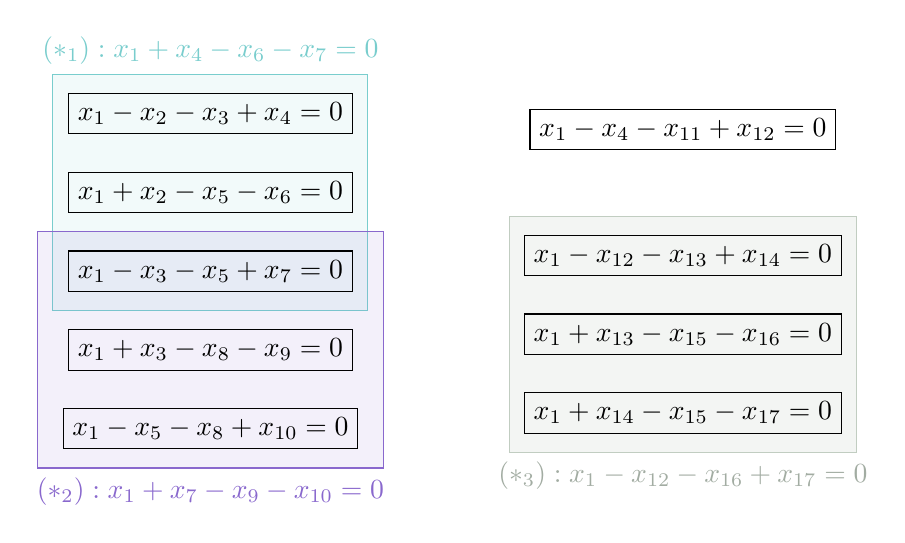
\begin{tikzpicture}

            \filldraw [fill = Honeydew3!20, draw = Honeydew3] (3.8, -4.3) rectangle (8.2, -1.3);
            \filldraw [fill = DarkSlateGray3!10, draw = DarkSlateGray3] (-2, -2.5) rectangle (2, 0.5);
            \fill [MediumPurple3!10] (-2.2, -4.5) rectangle (2.2, -1.5);
            \fill [MediumPurple3!50!DarkSlateGray3!20] (-2, -2.5) rectangle (2, -1.5);
            \draw [DarkSlateGray3!91!MediumPurple3] (-2, -1.5) -- (-2, -2.5) -- (2, -2.5) -- (2, -1.5);
            \draw [MediumPurple3] (-2.2, -4.5) rectangle (2.2, -1.5);

            \node [draw] at (0, 0) {$x_1 - x_2 - x_3 + x_4 = 0$};
            \node [draw] at (0, -1) {$x_1 + x_2 - x_5 - x_6 = 0$};
            \node [draw] at (0, -2) {$x_1 - x_3 - x_5 + x_7 = 0$};
            
            \node [DarkSlateGray3, anchor = south] at (0, 0.5) {$(*_1) : x_1 + x_4 - x_6 - x_7 = 0$};
            \node [draw] at (0, -3) {$x_1 + x_3 - x_8 - x_9 = 0$};
            \node [draw] at (0, -4) {$x_1 - x_5 - x_8 + x_{10} = 0$};
            
            \node [MediumPurple3, anchor = north] at (0, -4.5) {$(*_2) : x_1 + x_7 - x_9 - x_{10} = 0$};
            \node [draw] at (6, -0.2) {$x_1 - x_4 - x_{11} + x_{12} = 0$};
            \begin{scope}[yshift = -0.3cm]
                \node [draw] at (6, -1.5) {$x_1 - x_{12} - x_{13} + x_{14} = 0$};
                \node [draw] at (6, -2.5) {$x_1 + x_{13} - x_{15} - x_{16} = 0$};
                \node [draw] at (6, -3.5) {$x_1 + x_{14} - x_{15} - x_{17} = 0$};
                \node [Honeydew3!50!Honeydew4, anchor = north] at (6, -4) {$(*_3) : x_1 - x_{12} - x_{16} + x_{17} = 0$};
            \end{scope}
        \end{tikzpicture}
        \caption{This figure shows an example of a possible $\cS$ and the corresponding boxes. Here $i = 1$, and $\cS$ consists of the equations written in black. Each equation of $\cS$ is in a box of size $1$, and we have three boxes of size $3$, which are drawn in blue, purple, and green and labelled with the difference equalities that they minimally imply (named $(*_1)$, $(*_2)$, and $(*_3)$, respectively). For example, the blue box minimally implies $(*_1)$ because $(x_1 - x_2 - x_3 + x_4) + (x_1 + x_2 - x_5 - x_6) - (x_1 - x_3 - x_5 + x_7) = x_1 + x_4 - x_6 - x_7$.}
        \label{fig:boxes-config}
    \end{figure}

    We will work with the `connected components' of this picture, which we refer to as `blobs' --- to formalize this, consider the graph on $\cS$ in which two equations of $\cS$ are adjacent if and only if there is some box containing both of them. We say a \emph{blob} is a connected component of this graph, and the \emph{size} of a blob is again the number of equations it contains. In the example in Figure \ref{fig:boxes-config}, we have one blob of size $5$ (the union of the blue and purple boxes), one blob of size $3$ (the green box), and one blob of size $1$ (the one equation not in any big box). 

    Then the blobs form a partition of $\cS$ such that if $\cS$ $i$-certifies an index $j$, then in fact some blob must $i$-certify $j$ (every difference equality involving $x_i$ that is implied by $\cS$ is by definition implied by some box, and therefore by the blob containing this box). We will show that for each blob, the number of indices it $i$-certifies is at most twice its size.

    Clearly any blob of size $1$ can $i$-certify at most $2$ indices. Meanwhile, we will show that any blob of size $t > 1$ can only \emph{involve} at most $2t$ variables other than $x_i$, and therefore can $i$-certify at most $2t$ indices. 

    Any blob $\cT$ of size $t > 1$ can be written as a union of big boxes $\cT_0$, \ldots, $\cT_r$ such that for each $1 \leq p \leq r$, the box $\cT_p$ has nonempty intersection with $\cT_0 \cup \cdots \cup \cT_{p - 1}$. Let $t_0 = \abs{\cT_0}$, and for each $1 \leq p \leq r$, let $t_p = \abs{\cT_p \setminus (\cT_0 \cup \cdots \cup \cT_{p - 1})}$; then $t = t_0 + \cdots + t_r$. (Intuitively, we can imagine `building' $\cT$ by starting with some big box $\cT_0$, and then repeatedly adding in big boxes $\cT_1$, \ldots, $\cT_r$ such that at each step, the next big box we add overlaps with some previously added box; then for each $p$, we define $t_p$ as the number of new equations we add to the growing blob when we add in $\cT_p$. In the example in Figure \ref{fig:boxes-config}, for the blob of size $5$, we can take $\cT_0$ to be the blue box and $\cT_1$ to be the purple box; then $t_0 = 3$ and $t_1 = 2$.)

    First, Lemma \ref{lem:gen-min-impl}\ref{item:gmi-few-total} implies that $\cT_0$ contains at most $2t_0 + 2$ variables. Furthermore, equality cannot hold, as $x_i$ appears in all $t_0 + 1 \geq 3$ of the relevant equations, so in fact $\cT_0$ contains at most $2t_0 + 1$ variables. 

    Meanwhile, for each $1 \leq p \leq r$, Lemma \ref{lem:gen-min-impl}\ref{item:gmi-few-new} applied to $\cT_p \setminus (\cT_0 \cup \cdots \cup \cT_{p - 1})$ (which is a proper subset of $\cT_p$) gives that there are at most $2t_p$ variables that appear in $\cT_p$ but not $\cT_0 \cup \cdots \cup \cT_{p - 1}$. (Rephrased in terms of the process of building $\cT$ one box at a time, this states that when we add in the big box $\cT_p$ --- thus adding in $t_p$ new equations to our growing blob --- these $t_p$ new equations give us at most $2t_p$ new variables.) 
    
    So the total number of variables that appear in $\cT$ is at most \[(2t_0 + 1) + 2t_1 + \cdots + 2t_p = 2t + 1.\] Since one of these variables is $x_i$, this means at most $2t$ variables other than $x_i$ appear in $\cT$, as desired. 

    So for every blob, the number of indices it $i$-certifies is at most twice its size. Since the blobs form a partition of $\cS$, this means the \emph{total} number of indices $i$-certified by any blob is at most $2\abs{\cS}$, as desired. 
\end{proof}

Thus we have shown Lemma \ref{lem:2s-certify}, which completes the proof of Theorem \ref{thm:upper-bound} (our family of upper bounds on $g(n, k, \ell)$).  
\begin{thebibliography}{99}
  \bibitem[1]{Beh46}
  F.~A. Behrend.
  \newblock On sets of integers which contain no three terms in arithmetical
    progression.
  \newblock {\em Proceedings of the National Academy of Sciences},
    32(12):331--332, 1946.

  \bibitem[7]{Li22}
  Anqi Li.
  \newblock Progress on local properties problems of difference sets.
  \newblock {\em European Journal of Combinatorics}, 108(103618), 2022.

  \bibitem[8]{PS19}
  Cosmin Pohoata and Adam Sheffer.
  \newblock Local properties in colored graphs, distinct distances, and
    difference sets.
  \newblock {\em Combinatorica}, 39(3):705--714, 2019.

\end{thebibliography}\end{document}
